\documentclass[12pt,a4paper]{amsart}

\usepackage[slovene]{babel}
\usepackage[utf8]{inputenc}
\usepackage{amsmath,amssymb,amsfonts,bm}
\usepackage{url}
\usepackage{graphicx,subfig}
\usepackage{algorithmicx}
\usepackage{algpseudocode}





\textwidth 15cm
\textheight 24cm
\oddsidemargin.5cm
\evensidemargin.5cm
\topmargin-5mm
\addtolength{\footskip}{10pt}
\pagestyle{plain}
\overfullrule=15pt

\theoremstyle{definition}
\newtheorem{definicija}{Definicija}[section]
\newtheorem{primer}[definicija]{Primer}
\newtheorem{opomba}[definicija]{Opomba}

\theoremstyle{plain}
\newtheorem{lema}[definicija]{Lema}
\newtheorem{izrek}[definicija]{Izrek}
\newtheorem{trditev}[definicija]{Trditev}
\newtheorem{posledica}[definicija]{Posledica}

\newcommand{\N}{\mathbb N}
\newcommand{\R}{\mathbb R}

\begin{document}

% Naslovnica
%----------------------------------------------------------------------------------------------------
\thispagestyle{empty}
\noindent{\large
Univerza v Ljubljani\\[1mm]
Fakulteta za matematiko in fiziko\\[3mm]
Finančna matematika -- 1.~stopnja}
\vfill

\begin{center}{\large
Tilen Humar, Urban Rupnik\\[2mm]
{\Huge \bf Iskanje bitonične rešitve problema potujočega trgovca}\\[5mm]
Projekt OR pri predmetu Finančni praktikum\\[1cm]}
\end{center}
\vfill

\noindent{\large
Ljubljana, 2022}
\pagebreak

%----------------------------------------------------------------------------------------------------
\section{Predstavitev problema}

\noindent
{\bf Problem potujočega trgovca} oziroma {\bf problem trgovskega potnika} je ponavadi zastavljen v 
naslednji obliki.
\newline

\noindent
Obstaja $n$ mest, za katera poznamo razdalje med poljubnim parom mest. Trgovec želi obiskati vsa mesta, 
pri čemer pot začne in konča v istem mestu in vsak kraj obišče natanko enkrat. Katera je najkrajša 
oziroma najcenejša pot, ki jo lahko izbere trgovec?
\newline

\noindent
V matematičnem jeziku se problem torej prevede na iskanje najcenejšega Hamiltonovega cikla v polnem 
grafu $K_n$, kjer ima vsaka povezava $e$ znano utež (ceno) $c_e$. Ker pa je v osnovi dotični problem
``NP-težek'', to je, da bi za iskanje njegove rešitve potrebovali več kot polinomski čas, se omejimo na
lažjo nalogo iskanja njegove najkrajše bitonične rešitve.
\newline

\section{Bitonična pot}

\begin{definicija}
    Zaporedje $(x_n)_{n \in \N}$ je bitonično, ko obstaja tak $k, 1 \leq k < n$, da velja
    $$x_1 \leq x_2 \leq \cdots \leq x_k \geq \cdots \geq x_n.$$
\end{definicija}

\noindent
Bitonična rešitev problema, bo torej pot, kjer bomo začeli v skrajno levo ležečem vozlišču, nadaljevali strogo
desno do najbolj desnega vozlišča in še strogo levo nazaj do izhodišča. Bitoničnost poti lahko na grafu 
preverimo z navpičnicami. Vsaka navpična črta seka pot največ dvakrat.


\begin{figure}[!htb]%
    \centering
    \subfloat[\centering Bitonična pot]{{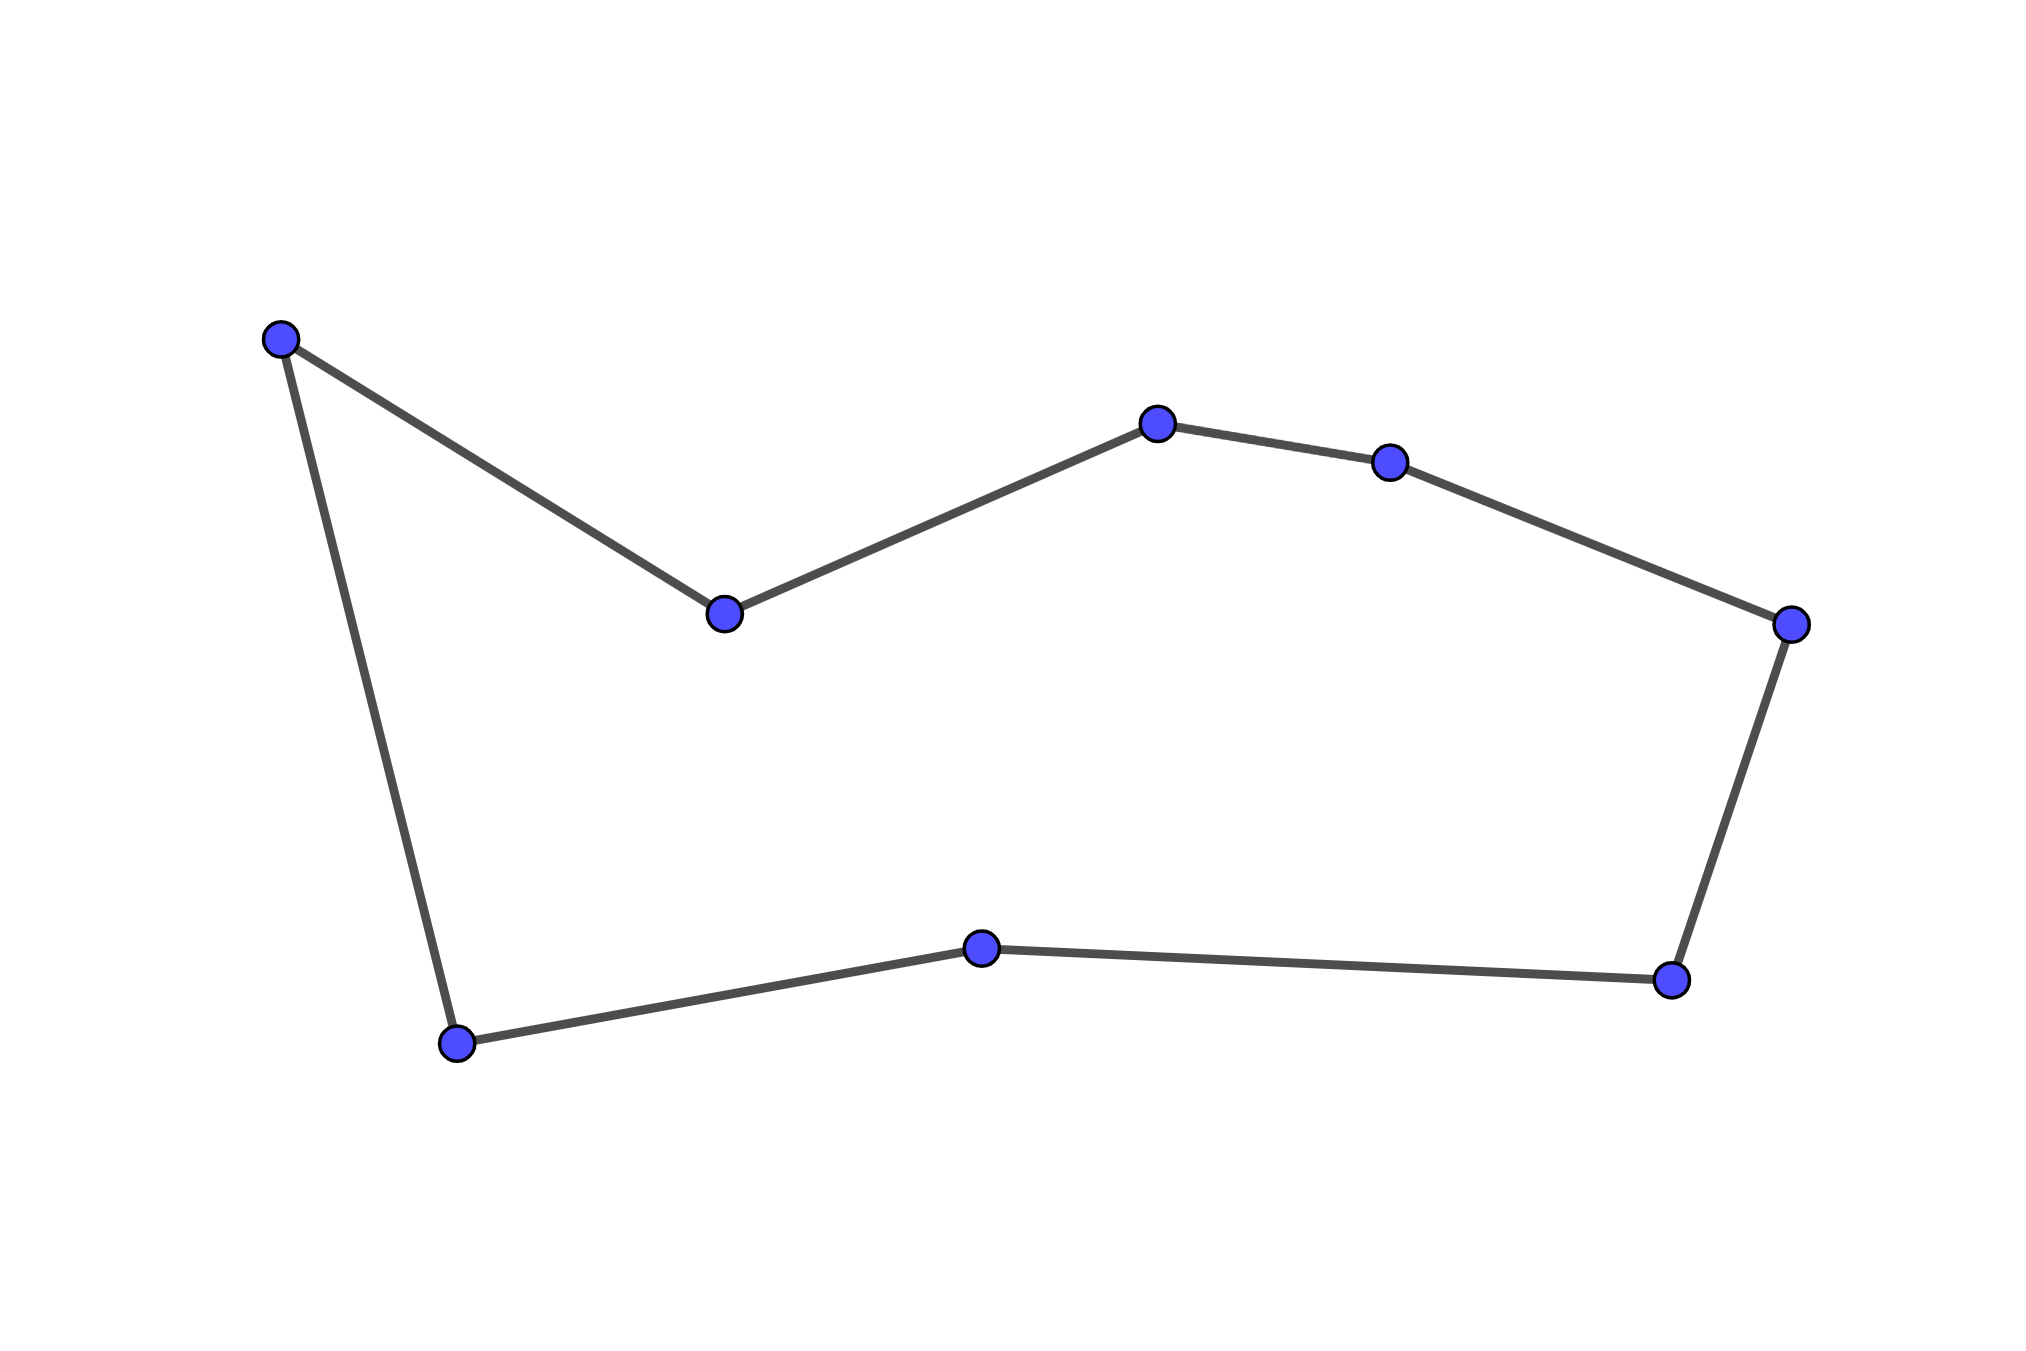
\includegraphics[width=6.9cm]{Slike grafov/graf1.png} }}%
    \qquad
    \subfloat[\centering Nebitonična pot]{{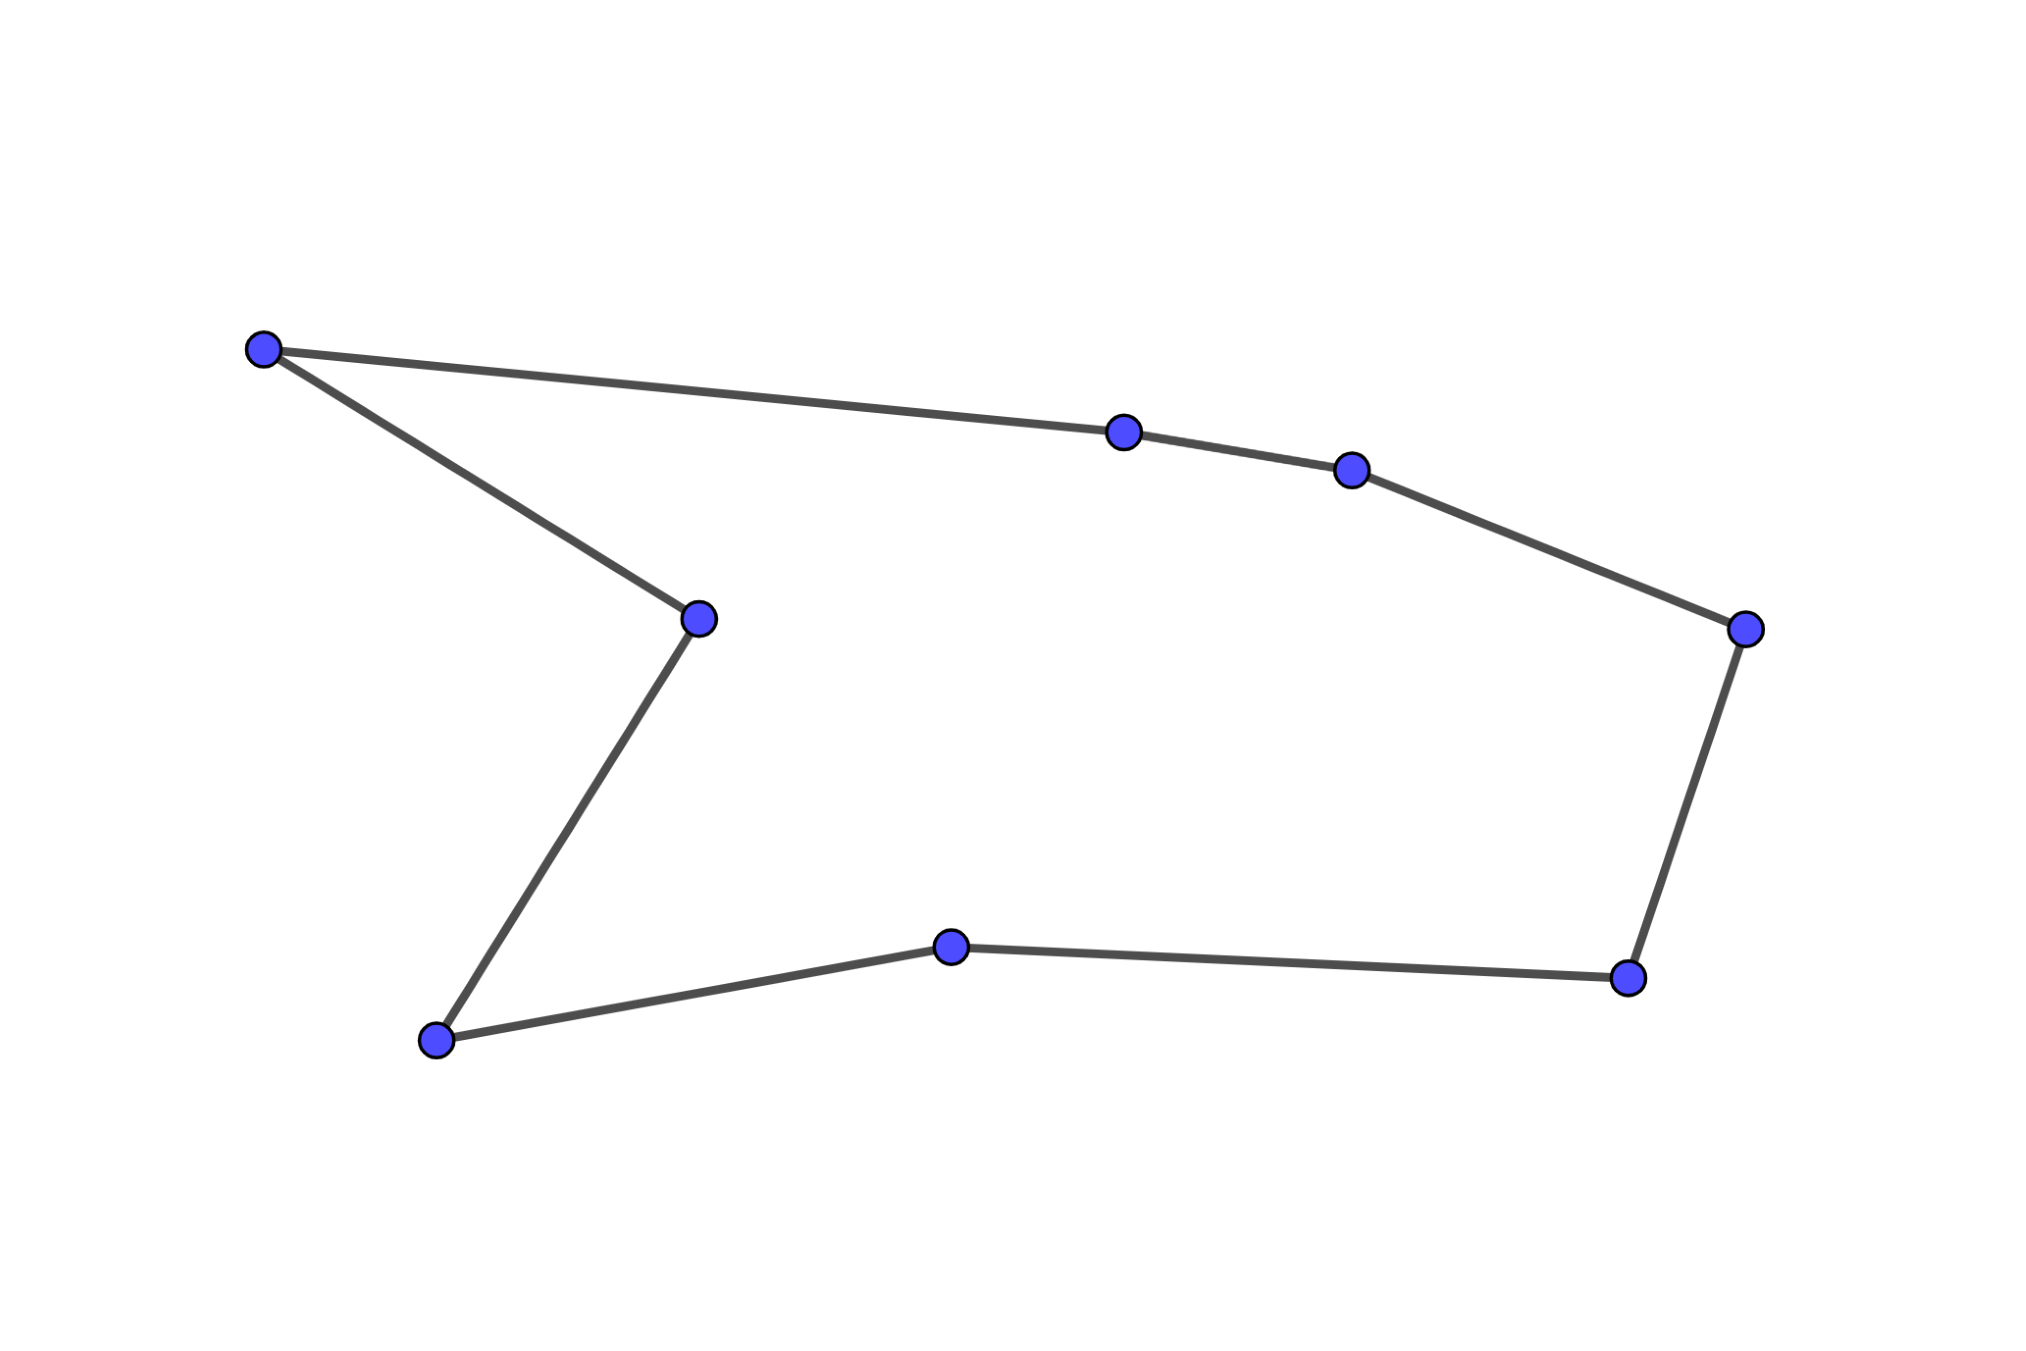
\includegraphics[width=6.9cm]{Slike grafov/graf2.png} }}%
    \caption{Primer bitonične in nebitonične poti na grafu}%
    \label{fig:example}%
\end{figure}


\noindent
Iskanje najkrajše bitonične poti je standardna naloga v dinamičnem programiranju, rešljiva v polinomskem
času $O(n^2),$ poznamo pa tudi hitrejši algoritem s časovno zahtevnostjo $O(n \log^2 n).$

\section{Dinamično programiranje}

\noindent
Imamo poln graf $K_n$ z množico $n$ vozlišč $\{v_1, v_2, \ldots, v_n\},$ urejenih po naraščajoči $x$ koordinati. 
Cene povezav so enake (evklidski) razdalji med posameznima vozliščema. Naš problem iskanja najkrajše 
bitonične poti (po definiciji dinamičnega programiranje) razdelimo na manjše probleme.
\newline

\noindent
Naj bo $P_{i,j}$ (za $i \leq j$) najkrajša bitonična pot, ki se začne v vozlišču $v_i$, nadaljuje strogo levo
do $v_1$ in nato strogo desno do $v_j$, kjer se konča. Slednja pot obišče vozlišča $\{v_1, v_2, \ldots, v_j\}.$ Rešitev
problema potujočega trgovca bo torej pot $P_{n,n}$ oziroma $P_{n-1, n} + e_{n-1, n},$ kjer
je $e_{n-1, n}$ povezava med $v_{n-1}$ in $v_{n}.$ Razčlenimo do zdaj ugotovljeno na nekaj podprimerov, iz
česar bomo izpeljali rekurzivno formulo.
\newline

\noindent
Naj za pot $P_{i,j}$ velja $\bm{i < j - 1}$. V slednji poti bo tako $v_{j-1}$ predhodnik $v_j,$ zato velja,
če iz poti $P_{i,j}$ odstranimo povezavo $e_{j-1,j},$ dobimo rešitev $P_{i, j-1}.$
\newline

\noindent
Na spodnji sliki \ref{slika:1. primer} je izrisan primer poti $P_{5,8}$, kjer omenjena neenakost velja
($5 < 8 - 1$). Ko smo na poti odstranili povezavo $e_{7,8}$, nam je ostala ravno pot $P_{5,7}$ (desna slika).

\begin{figure}[!htb]%
  \centering
  \subfloat[\centering Graf $P_{5,8}$]{{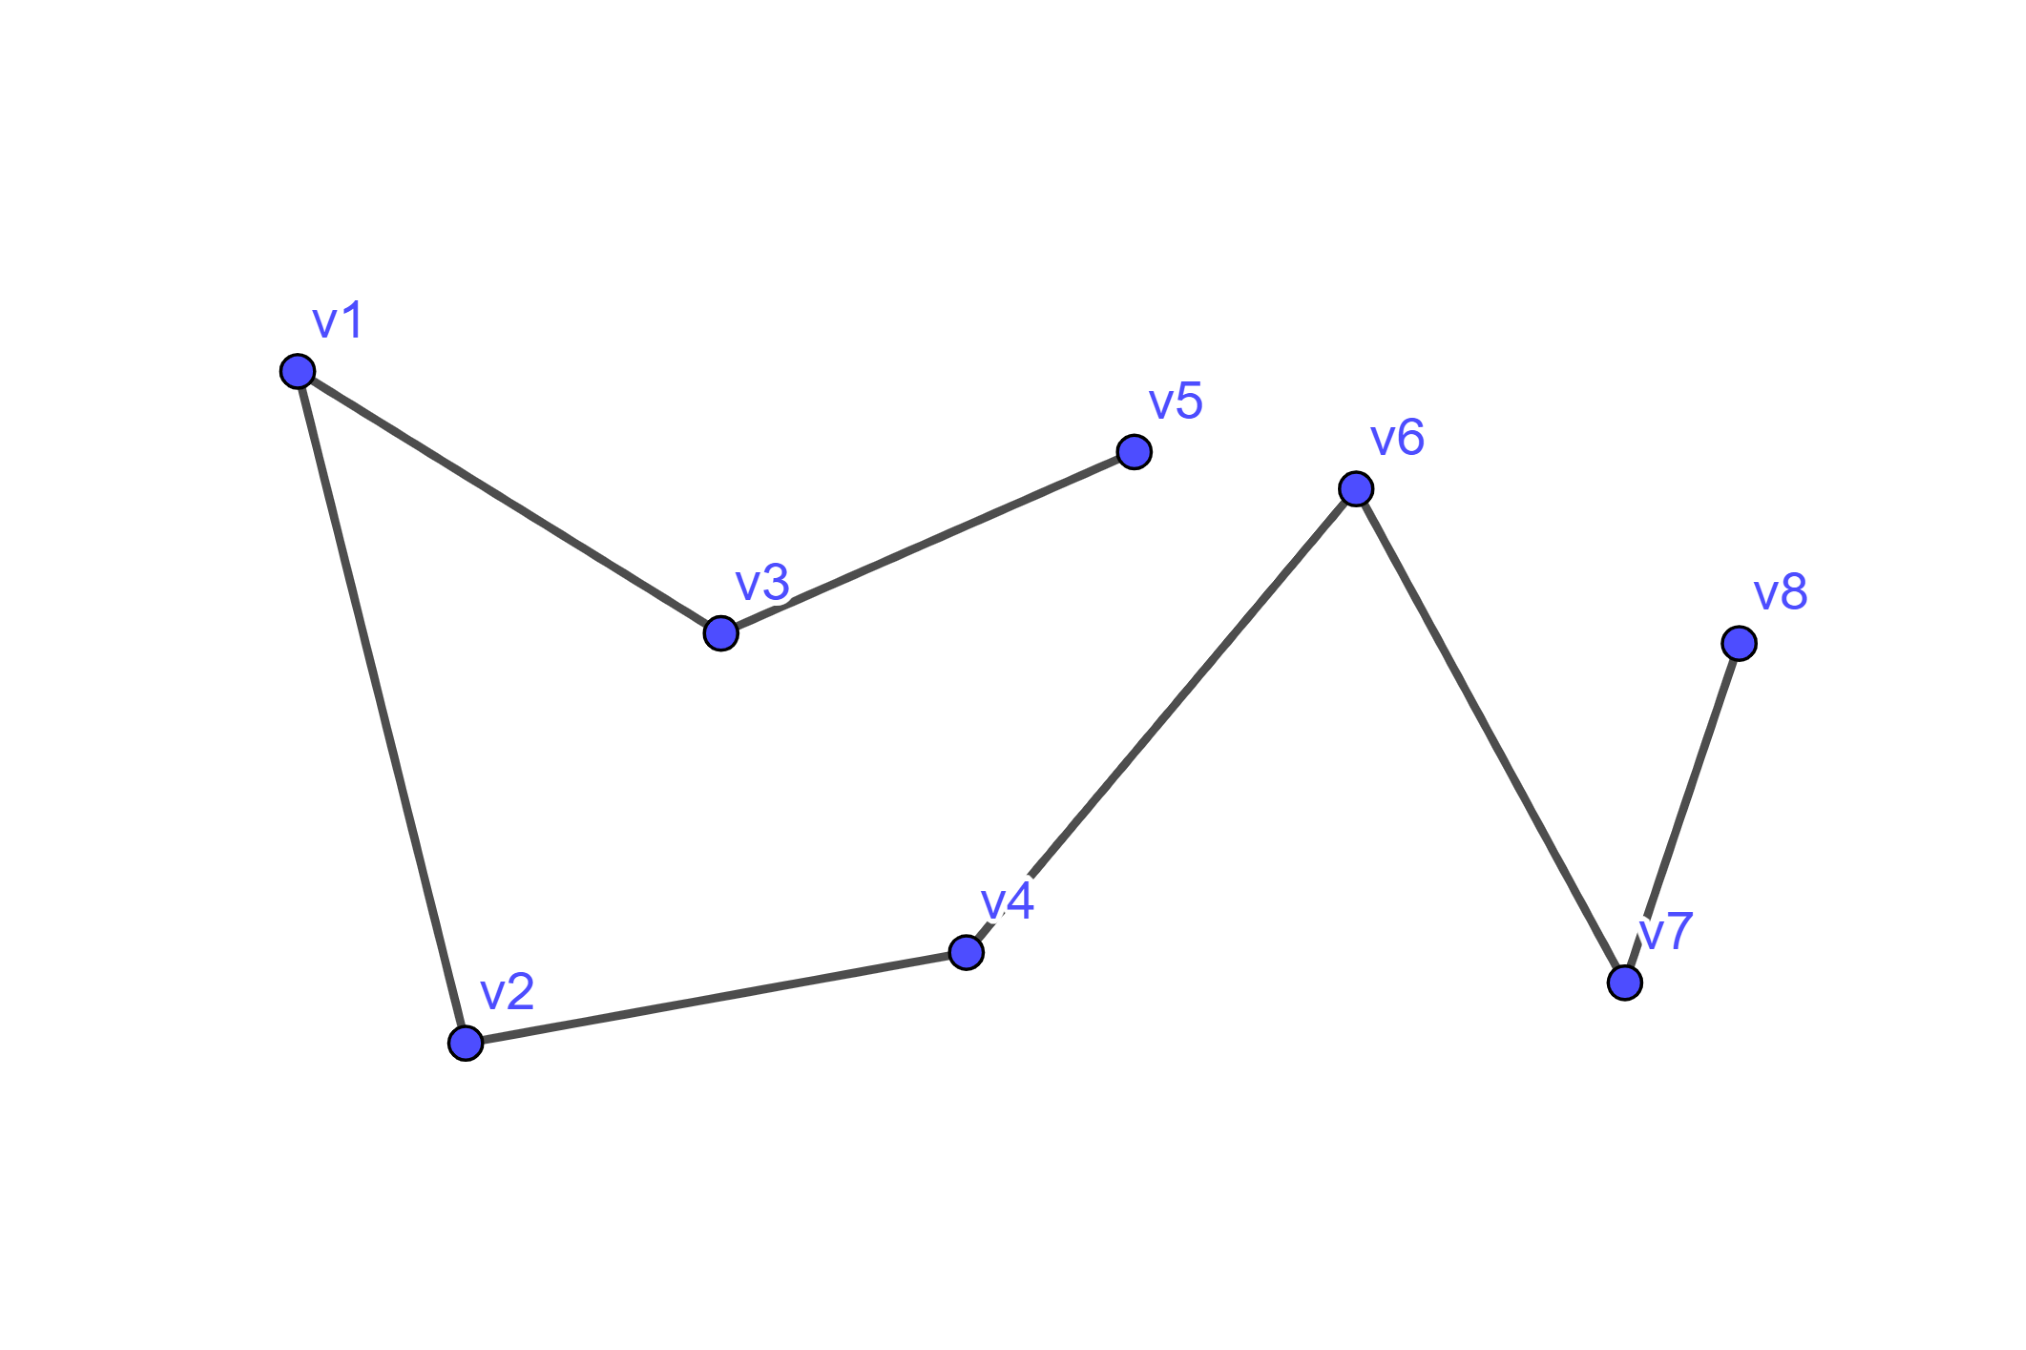
\includegraphics[width=6.9cm]{Slike grafov/graf3.png} }}%
  \qquad
  \subfloat[\centering Graf $P_{5,7}$]{{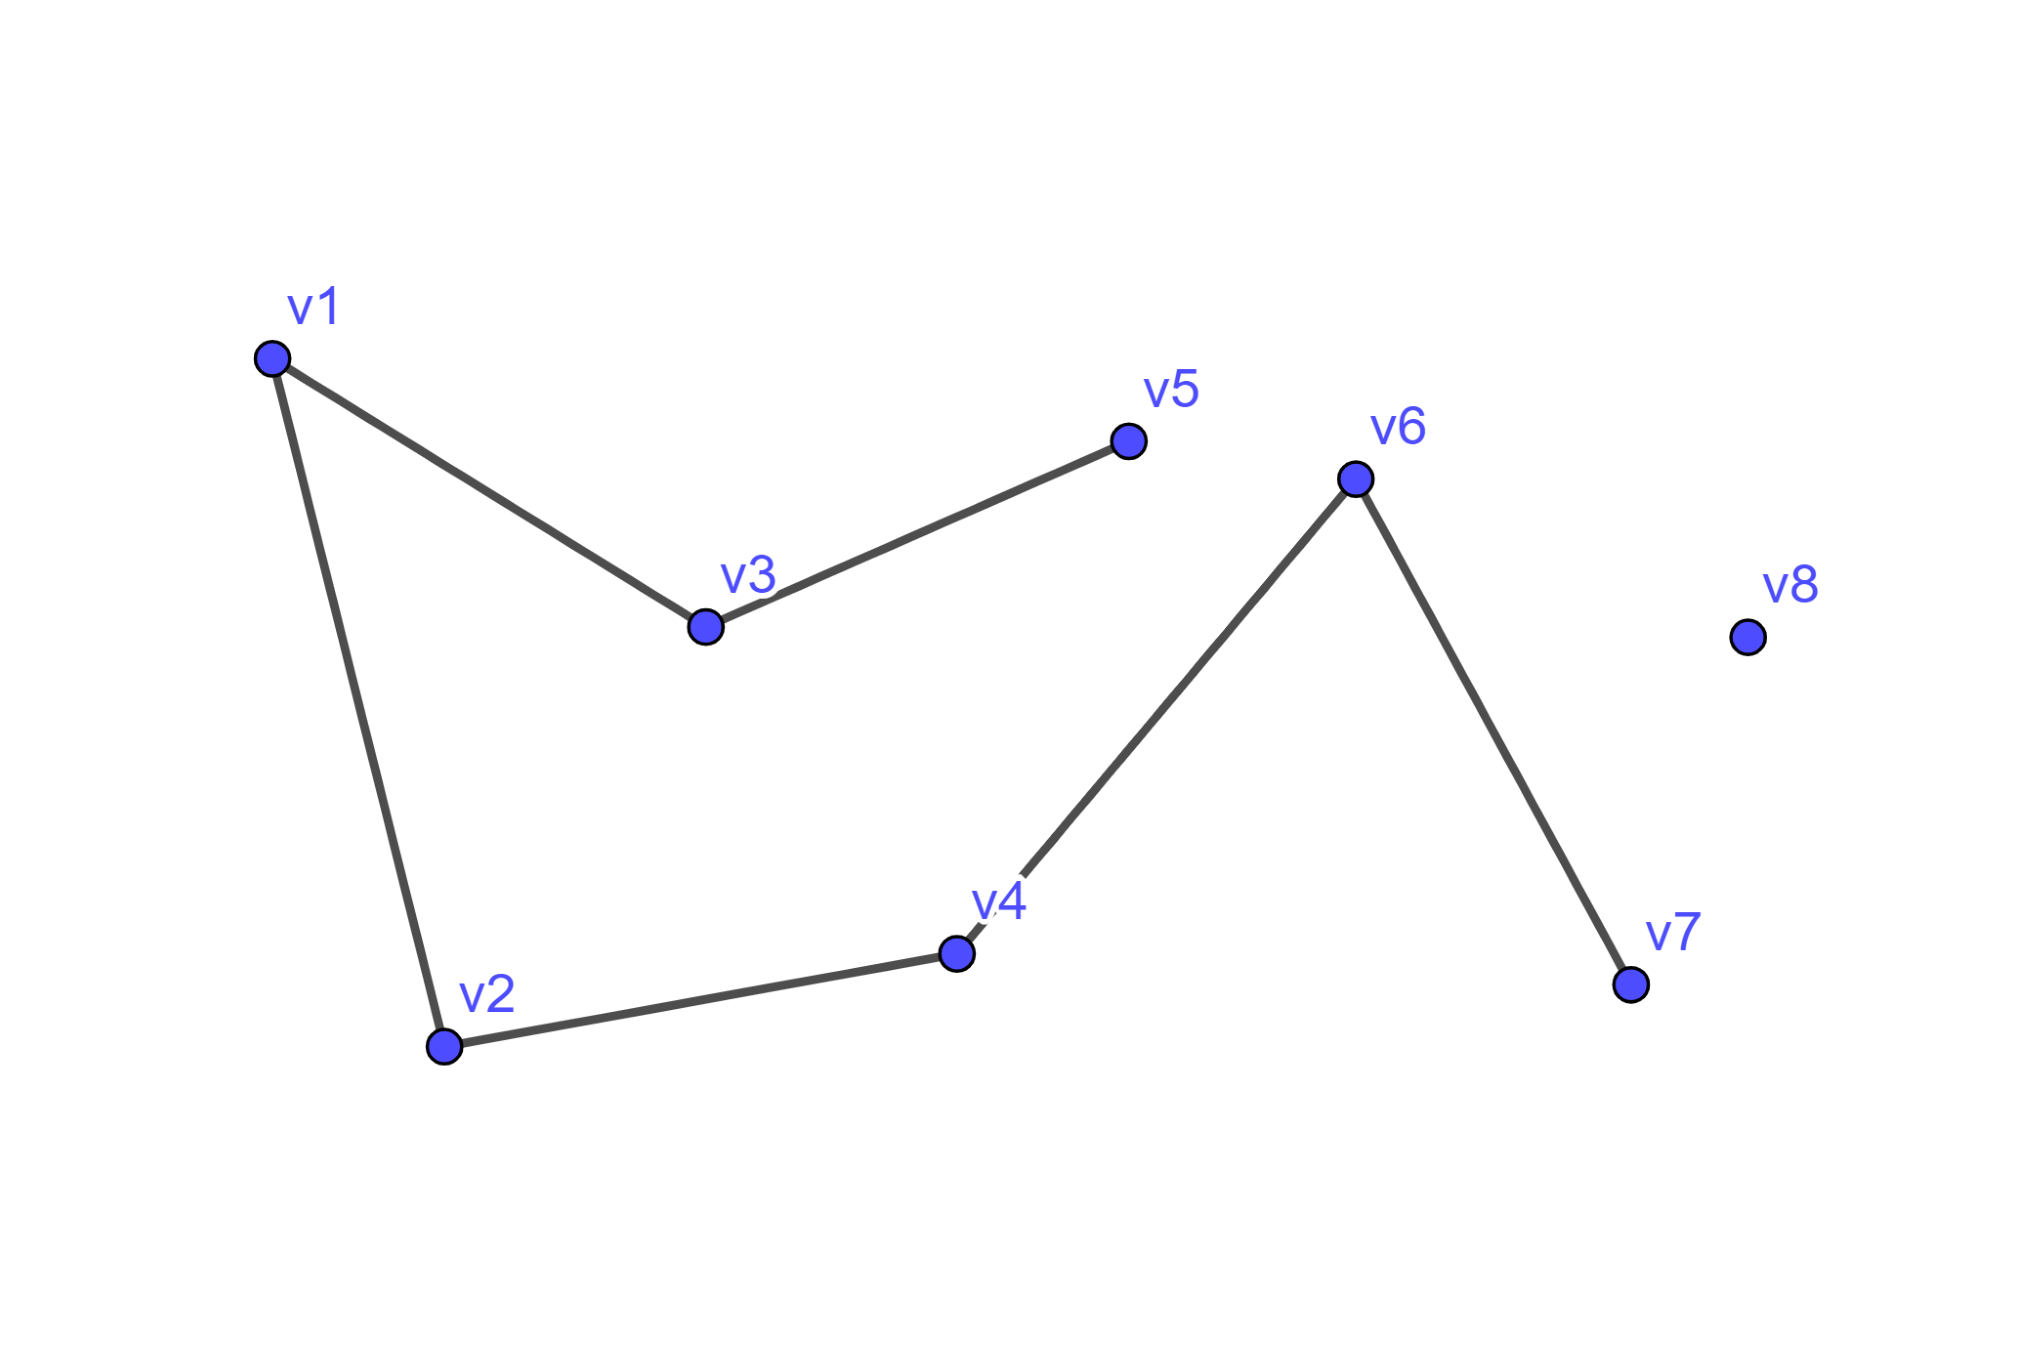
\includegraphics[width=6.9cm]{Slike grafov/graf4.png} }}%
  \caption{Primer grafov poti $P_{i,j}$ za $i < j - 1.$}%
  \label{slika:1. primer}%
\end{figure}


\noindent
Poglejmo še primer, ko za $P_{i, j}$ velja $\bm{i = j - 1}$. Na poti $P_{i,j}$ bo imela točka $v_j$ predhodnika
$v_k$ za $1 \leq k \leq j - 2.$ Če sedaj odstranimo povezavo $e_{k,j}$ nam ostane pot $P_{k, j-1}.$
\newline

\begin{figure}[!htb]%
  \centering
  \subfloat[\centering Graf $P_{6,7}$]{{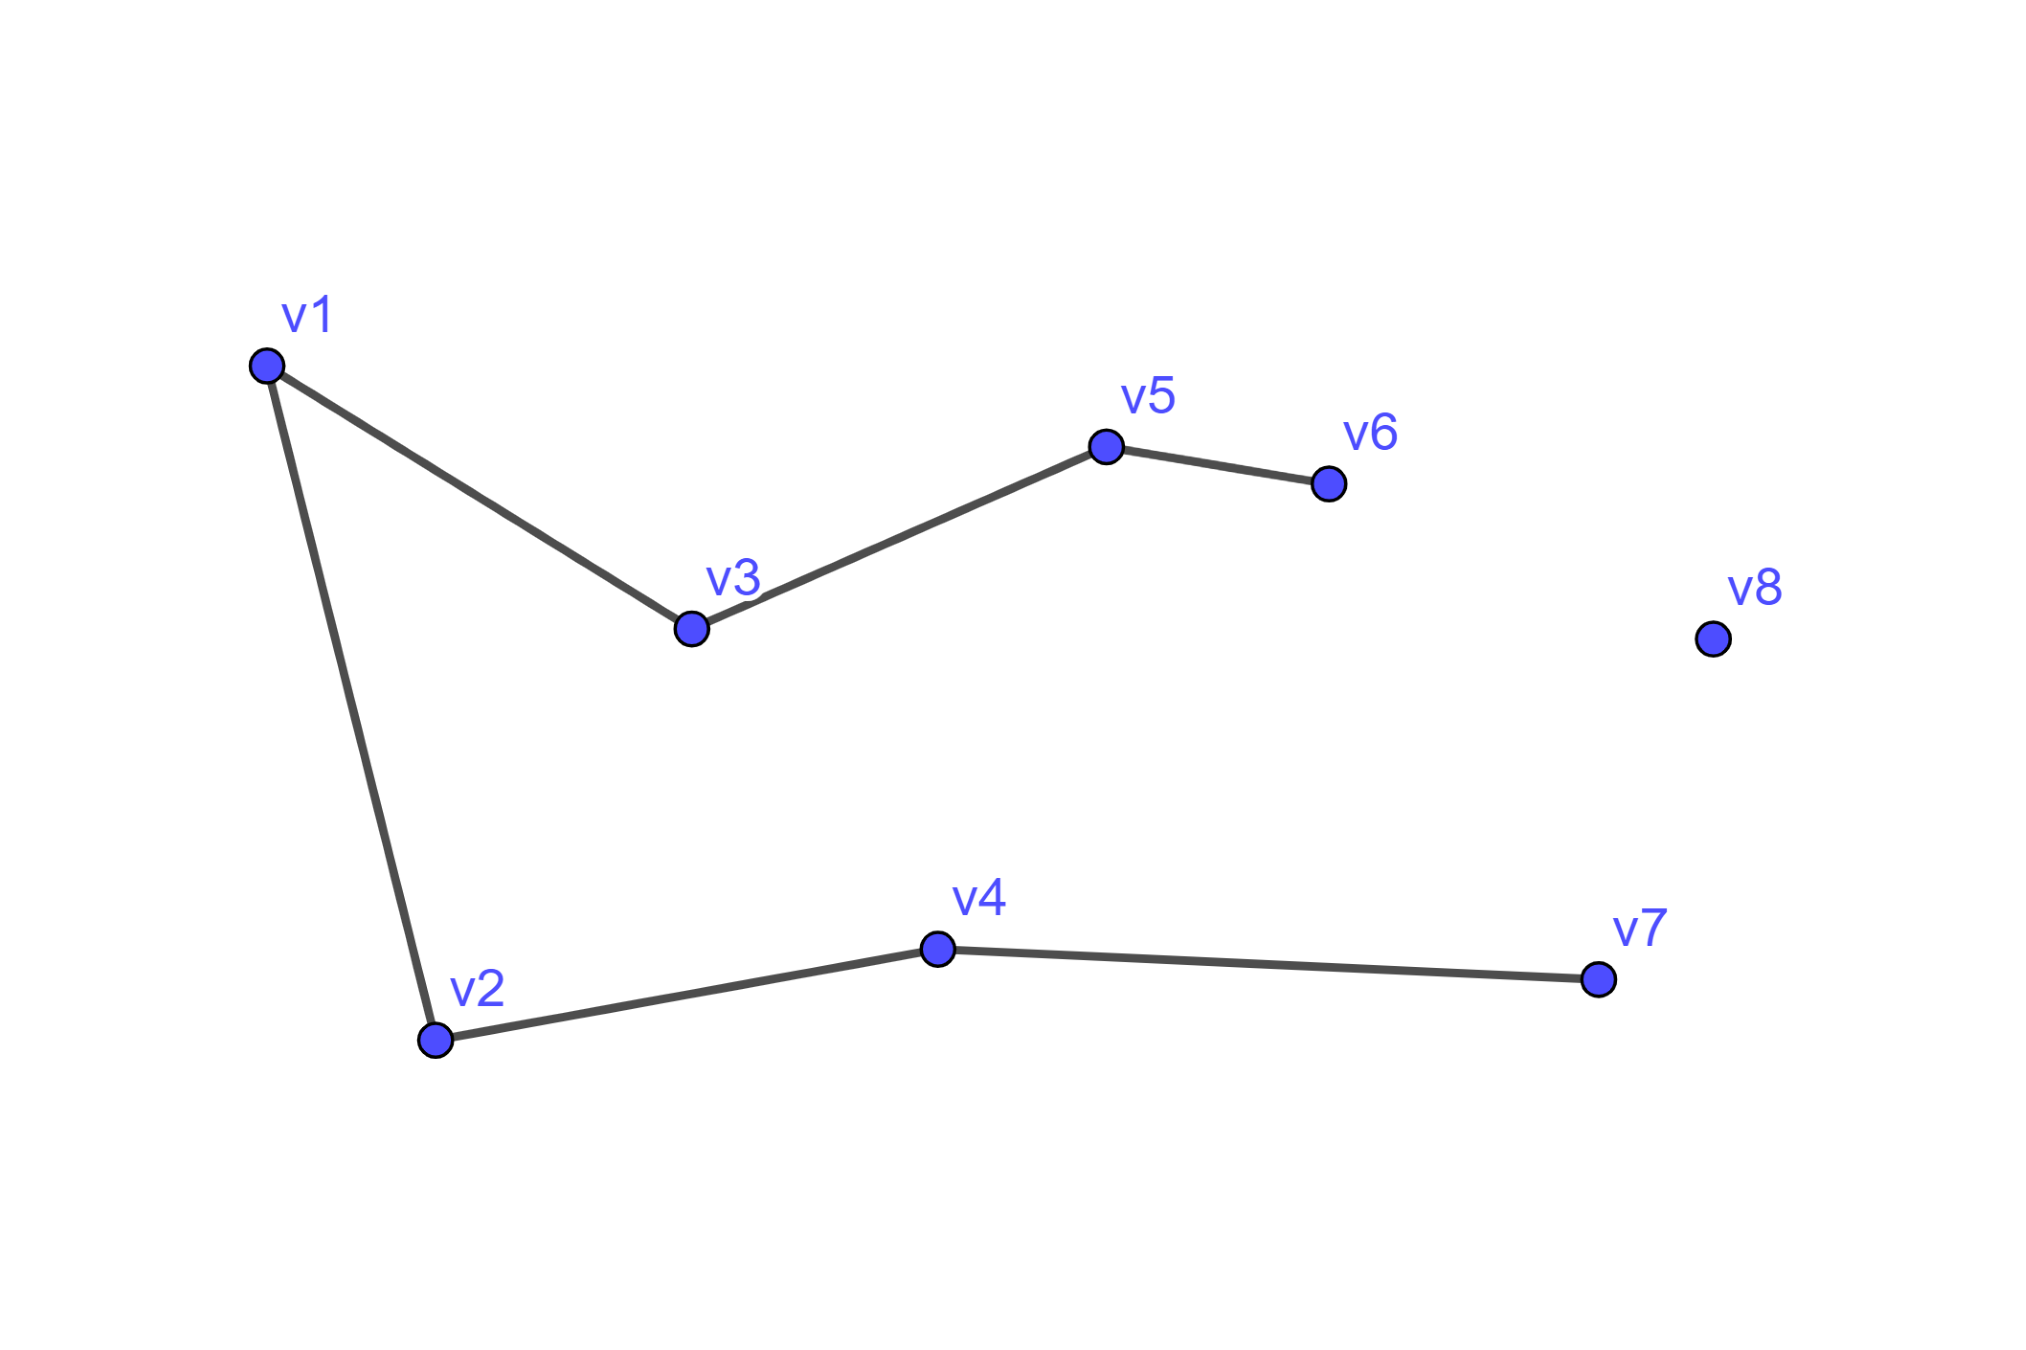
\includegraphics[width=6.9cm]{Slike grafov/graf5.png} }}%
  \qquad
  \subfloat[\centering Graf $P_{4,6}$]{{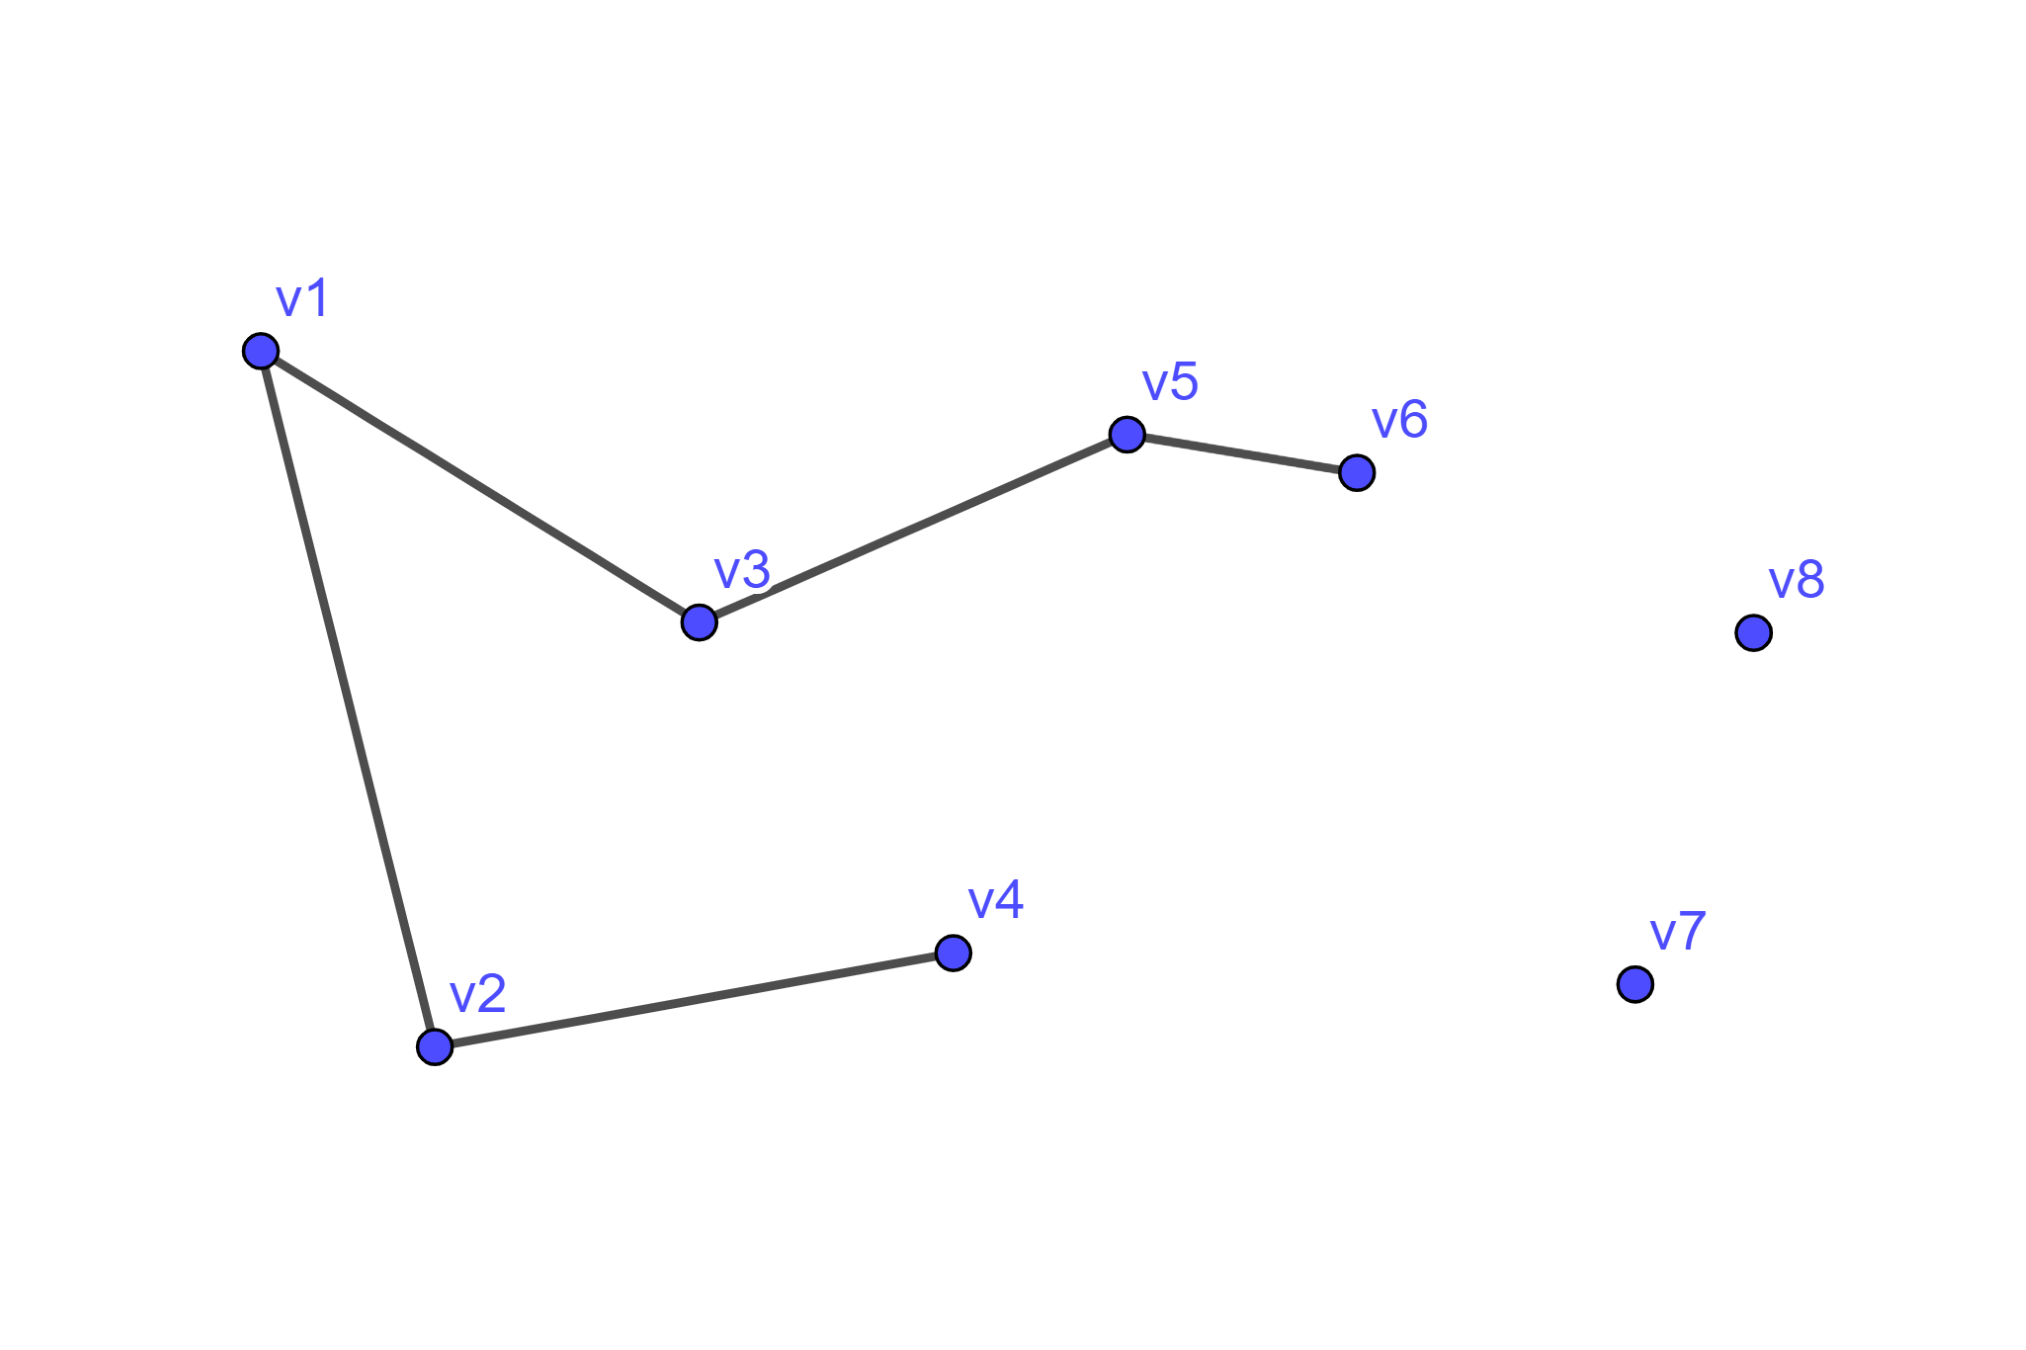
\includegraphics[width=6.9cm]{Slike grafov/graf6.png} }}%
  \caption{Primer grafov poti $P_{i,j} $ za $i = j - 1$}%
  \label{slika:2. primer}%
\end{figure}

\noindent
Slednji primer je prikazan na sliki \ref{slika:2. primer}. Za pot $P_{6,7}$ velja enakost ($6 = 7 - 1$), 
torej ima vozlišče $v_7$ predhodnika $v_k$ (za $1 \leq k \leq 7 - 2$). V našem primeru je $k = 4$ in ko 
iz poti $P_{6,7}$ odstranimo povezavo $e_{4,7},$ dobimo ravno pot $P_{4,6}.$
\newline

\noindent
V zadnji primer ($i = j - 1$) spada tudi skrajni dogodek $\bm{i = 1}$ in $\bm{j = 2}$. Imamo pot z le dvema
vozliščema, torej je ta enaka kar njuni povezavi $P_{1,2} = e_{1,2}.$
\newline

\noindent
Zgornje izpeljave lahko sedaj združimo v rekurzivno formulo.


\begin{equation*}
    P_{i,j} =
      \begin{cases}
        e_{1, 2} & \text{$i = 1$, $j = 2$}\\
        P_{i, j-1} + e_{j-1, j} & \text{$i < j - 1$}\\
        \displaystyle \min_{1 \leq k \leq j - 2} P_{k, j-1} + e_{k, j} & \text{$i = j - 1$}
      \end{cases}   
      \newline      
  \end{equation*}

\section{Program}

\noindent
V programskem jeziku R, sva pripravila program, ki vsebuje:

\begin{itemize}
  \item funkcijo za generiranje točk v $\R^2$ (predpostavka: $x$ koordinate so različna
  cela števila, $y$ pa poljubna realna)
  \item funkcijo za risanje točk
  \item funkcijo za izračun evklidske razdalje med točkama
  \item program za iskanje najkrajše bitonične poti
  \item funkcijo za izpis poti
  \newline
\end{itemize}


\noindent
Program za iskanje najkrajše bitonične poti lahko, v rahlo poenostavljeni obliki, predstavimo z naslednjo
psevdokodo.
\newline




\end{document}